% Options for packages loaded elsewhere
\PassOptionsToPackage{unicode}{hyperref}
\PassOptionsToPackage{hyphens}{url}
%
\documentclass[
  man]{apa6}
\usepackage{amsmath,amssymb}
\usepackage{lmodern}
\usepackage{iftex}
\ifPDFTeX
  \usepackage[T1]{fontenc}
  \usepackage[utf8]{inputenc}
  \usepackage{textcomp} % provide euro and other symbols
\else % if luatex or xetex
  \usepackage{unicode-math}
  \defaultfontfeatures{Scale=MatchLowercase}
  \defaultfontfeatures[\rmfamily]{Ligatures=TeX,Scale=1}
\fi
% Use upquote if available, for straight quotes in verbatim environments
\IfFileExists{upquote.sty}{\usepackage{upquote}}{}
\IfFileExists{microtype.sty}{% use microtype if available
  \usepackage[]{microtype}
  \UseMicrotypeSet[protrusion]{basicmath} % disable protrusion for tt fonts
}{}
\makeatletter
\@ifundefined{KOMAClassName}{% if non-KOMA class
  \IfFileExists{parskip.sty}{%
    \usepackage{parskip}
  }{% else
    \setlength{\parindent}{0pt}
    \setlength{\parskip}{6pt plus 2pt minus 1pt}}
}{% if KOMA class
  \KOMAoptions{parskip=half}}
\makeatother
\usepackage{xcolor}
\IfFileExists{xurl.sty}{\usepackage{xurl}}{} % add URL line breaks if available
\IfFileExists{bookmark.sty}{\usepackage{bookmark}}{\usepackage{hyperref}}
\hypersetup{
  pdftitle={My new demo of a semester long project},
  pdfauthor={Matthew Crump1},
  pdflang={en-EN},
  pdfkeywords={Stroop, Posture, Reproducible analysis},
  hidelinks,
  pdfcreator={LaTeX via pandoc}}
\urlstyle{same} % disable monospaced font for URLs
\usepackage{graphicx}
\makeatletter
\def\maxwidth{\ifdim\Gin@nat@width>\linewidth\linewidth\else\Gin@nat@width\fi}
\def\maxheight{\ifdim\Gin@nat@height>\textheight\textheight\else\Gin@nat@height\fi}
\makeatother
% Scale images if necessary, so that they will not overflow the page
% margins by default, and it is still possible to overwrite the defaults
% using explicit options in \includegraphics[width, height, ...]{}
\setkeys{Gin}{width=\maxwidth,height=\maxheight,keepaspectratio}
% Set default figure placement to htbp
\makeatletter
\def\fps@figure{htbp}
\makeatother
\setlength{\emergencystretch}{3em} % prevent overfull lines
\providecommand{\tightlist}{%
  \setlength{\itemsep}{0pt}\setlength{\parskip}{0pt}}
\setcounter{secnumdepth}{-\maxdimen} % remove section numbering
% Make \paragraph and \subparagraph free-standing
\ifx\paragraph\undefined\else
  \let\oldparagraph\paragraph
  \renewcommand{\paragraph}[1]{\oldparagraph{#1}\mbox{}}
\fi
\ifx\subparagraph\undefined\else
  \let\oldsubparagraph\subparagraph
  \renewcommand{\subparagraph}[1]{\oldsubparagraph{#1}\mbox{}}
\fi
\newlength{\cslhangindent}
\setlength{\cslhangindent}{1.5em}
\newlength{\csllabelwidth}
\setlength{\csllabelwidth}{3em}
\newlength{\cslentryspacingunit} % times entry-spacing
\setlength{\cslentryspacingunit}{\parskip}
\newenvironment{CSLReferences}[2] % #1 hanging-ident, #2 entry spacing
 {% don't indent paragraphs
  \setlength{\parindent}{0pt}
  % turn on hanging indent if param 1 is 1
  \ifodd #1
  \let\oldpar\par
  \def\par{\hangindent=\cslhangindent\oldpar}
  \fi
  % set entry spacing
  \setlength{\parskip}{#2\cslentryspacingunit}
 }%
 {}
\usepackage{calc}
\newcommand{\CSLBlock}[1]{#1\hfill\break}
\newcommand{\CSLLeftMargin}[1]{\parbox[t]{\csllabelwidth}{#1}}
\newcommand{\CSLRightInline}[1]{\parbox[t]{\linewidth - \csllabelwidth}{#1}\break}
\newcommand{\CSLIndent}[1]{\hspace{\cslhangindent}#1}
\ifLuaTeX
\usepackage[bidi=basic]{babel}
\else
\usepackage[bidi=default]{babel}
\fi
\babelprovide[main,import]{english}
% get rid of language-specific shorthands (see #6817):
\let\LanguageShortHands\languageshorthands
\def\languageshorthands#1{}
% Manuscript styling
\usepackage{upgreek}
\captionsetup{font=singlespacing,justification=justified}

% Table formatting
\usepackage{longtable}
\usepackage{lscape}
% \usepackage[counterclockwise]{rotating}   % Landscape page setup for large tables
\usepackage{multirow}		% Table styling
\usepackage{tabularx}		% Control Column width
\usepackage[flushleft]{threeparttable}	% Allows for three part tables with a specified notes section
\usepackage{threeparttablex}            % Lets threeparttable work with longtable

% Create new environments so endfloat can handle them
% \newenvironment{ltable}
%   {\begin{landscape}\begin{center}\begin{threeparttable}}
%   {\end{threeparttable}\end{center}\end{landscape}}
\newenvironment{lltable}{\begin{landscape}\begin{center}\begin{ThreePartTable}}{\end{ThreePartTable}\end{center}\end{landscape}}

% Enables adjusting longtable caption width to table width
% Solution found at http://golatex.de/longtable-mit-caption-so-breit-wie-die-tabelle-t15767.html
\makeatletter
\newcommand\LastLTentrywidth{1em}
\newlength\longtablewidth
\setlength{\longtablewidth}{1in}
\newcommand{\getlongtablewidth}{\begingroup \ifcsname LT@\roman{LT@tables}\endcsname \global\longtablewidth=0pt \renewcommand{\LT@entry}[2]{\global\advance\longtablewidth by ##2\relax\gdef\LastLTentrywidth{##2}}\@nameuse{LT@\roman{LT@tables}} \fi \endgroup}

% \setlength{\parindent}{0.5in}
% \setlength{\parskip}{0pt plus 0pt minus 0pt}

% Overwrite redefinition of paragraph and subparagraph by the default LaTeX template
% See https://github.com/crsh/papaja/issues/292
\makeatletter
\renewcommand{\paragraph}{\@startsection{paragraph}{4}{\parindent}%
  {0\baselineskip \@plus 0.2ex \@minus 0.2ex}%
  {-1em}%
  {\normalfont\normalsize\bfseries\itshape\typesectitle}}

\renewcommand{\subparagraph}[1]{\@startsection{subparagraph}{5}{1em}%
  {0\baselineskip \@plus 0.2ex \@minus 0.2ex}%
  {-\z@\relax}%
  {\normalfont\normalsize\itshape\hspace{\parindent}{#1}\textit{\addperi}}{\relax}}
\makeatother

% \usepackage{etoolbox}
\makeatletter
\patchcmd{\HyOrg@maketitle}
  {\section{\normalfont\normalsize\abstractname}}
  {\section*{\normalfont\normalsize\abstractname}}
  {}{\typeout{Failed to patch abstract.}}
\patchcmd{\HyOrg@maketitle}
  {\section{\protect\normalfont{\@title}}}
  {\section*{\protect\normalfont{\@title}}}
  {}{\typeout{Failed to patch title.}}
\makeatother
\keywords{Stroop, Posture, Reproducible analysis\newline\indent Word count: 1000}
\DeclareDelayedFloatFlavor{ThreePartTable}{table}
\DeclareDelayedFloatFlavor{lltable}{table}
\DeclareDelayedFloatFlavor*{longtable}{table}
\makeatletter
\renewcommand{\efloat@iwrite}[1]{\immediate\expandafter\protected@write\csname efloat@post#1\endcsname{}}
\makeatother
\usepackage{lineno}

\linenumbers
\usepackage{csquotes}
\usepackage[titles]{tocloft}
\cftpagenumbersoff{figure}
\renewcommand{\cftfigpresnum}{\itshape\figurename\enspace}
\renewcommand{\cftfigaftersnum}{.\space}
\setlength{\cftfigindent}{0pt}
\setlength{\cftafterloftitleskip}{0pt}
\settowidth{\cftfignumwidth}{Figure 10.\qquad}
\ifLuaTeX
  \usepackage{selnolig}  % disable illegal ligatures
\fi

\title{My new demo of a semester long project}
\author{Matthew Crump\textsuperscript{1}}
\date{}


\shorttitle{Semester project}

\authornote{

Matthew J. C. Crump, Department of Psychology, Brooklyn College of the City University of New York, and Graduate Center of the City University of New York.

Correspondence concerning this article should be addressed to Matthew Crump, 2900 Bedford Avenue. E-mail: \href{mailto:mcrump@brooklyn.cuny.edu}{\nolinkurl{mcrump@brooklyn.cuny.edu}}

}

\affiliation{\vspace{0.5cm}\textsuperscript{1} Brooklyn College}

\abstract{
This is a demo for the semester long project in PSYC 7765/66.
}



\begin{document}
\maketitle

This is a short example of creating an APA manuscript using papaja. It is intended to provide example code for your semester project. This would normally be the introduction to your paper. Below is a very brief introduction.

This report reproduces the analysis of Experiment 3 reported in Rosenbaum, Mama, and Algom (2017). The data were downloaded from \url{https://osf.io/b7x8q/}

Rosenbaum et al. (2017) had participants perform a Stroop task (Bugg \& Crump, 2012; for a review see, MacLeod, 1991) in one of two posture conditions. Participants either sat and performed the Stroop task, or stood and performed the Stroop task. The question was whether the size of the Stroop effect would change as a function of posture. The Stroop effect is measured as a difference between reaction times on congruent vs.~incongruent trials.The experiment involved a 2 (Posture: sitting vs standing) x 2 (congruency: congruent vs.~incongruent) repeated measures design.

\hypertarget{methods}{%
\section{Methods}\label{methods}}

\hypertarget{participants}{%
\subsection{Participants}\label{participants}}

There were 50 participants

\hypertarget{material}{%
\subsection{Material}\label{material}}

The details of the Stroop experiment are report in the paper (Rosenbaum et al., 2017).

\hypertarget{procedure}{%
\subsection{Procedure}\label{procedure}}

In each posture condition, participants completed 72 Stroop trials, half congruent and half incongruent.

\hypertarget{results}{%
\section{Results}\label{results}}

First, the means for each condition collapsed across subjects are presented in Table 1.

\begin{table}[tbp]

\begin{center}
\begin{threeparttable}

\caption{\label{tab:unnamed-chunk-1}}

\begin{tabular}{llll}
\toprule
Congruency & \multicolumn{1}{c}{Posture} & \multicolumn{1}{c}{mean\_RT} & \multicolumn{1}{c}{SEM}\\
\midrule
Congruent & Sit & 821.92 & 16.60\\
Congruent & Stand & 807.96 & 14.94\\
Incongruent & Sit & 940.79 & 17.91\\
Incongruent & Stand & 903.91 & 15.35\\
\bottomrule
\end{tabular}

\end{threeparttable}
\end{center}

\end{table}

Additionally, the means for each condition are plotted in Figure 1.

\begin{figure}
\centering
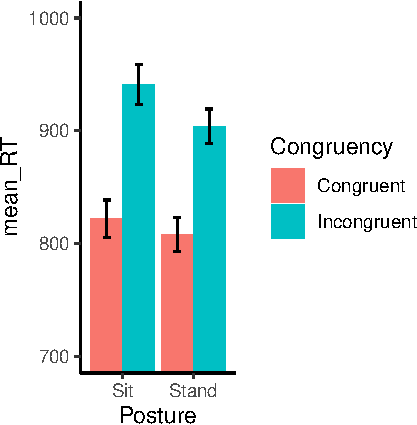
\includegraphics{SemesterProject_files/figure-latex/unnamed-chunk-2-1.pdf}
\caption{\label{fig:unnamed-chunk-2}Mean reaction times as a function of Congruency and Posture conditions, with standard errors of the mean.}
\end{figure}

The original authors reported the following in their analysis, ``The Stroop effects in both the sitting condition, M = 118.9 ms, t(49) = 16.52, p \textless{} .01, d = 2.376, and the standing condition, M = 95.9 ms, t(49) = 14.327, p \textless{} .01, d = 2.034.''

Open data from this paper was obtained, and a script was generated to attempt a reproduction of the analysis. The following results are generated by the R analysis script.

The re-analysis for the sitting Stroop effect showed a significant Stroop effect, \(M_d = 118.86\), 95\% CI \([104.40, 133.33]\), \(t(49) = 16.52\), \(p < .001\). The re-analysis for the standing Stroop effect was significant, \(M_d = 95.95\), 95\% CI \([82.49, 109.41]\), \(t(49) = 14.33\), \(p < .001\).

Here are a few more examples of using R snippets in text. Remember, this is not an R code chunk. This is regular text. Here is an example of using an R snippet to print the addition of 1+1 = 2.

\hypertarget{power-analysis}{%
\section{Power analysis}\label{power-analysis}}

The following reports a power curve analysis for one the t-tests in the design. This shows the power of the design to detect effects of different sizes.

\begin{figure}
\centering
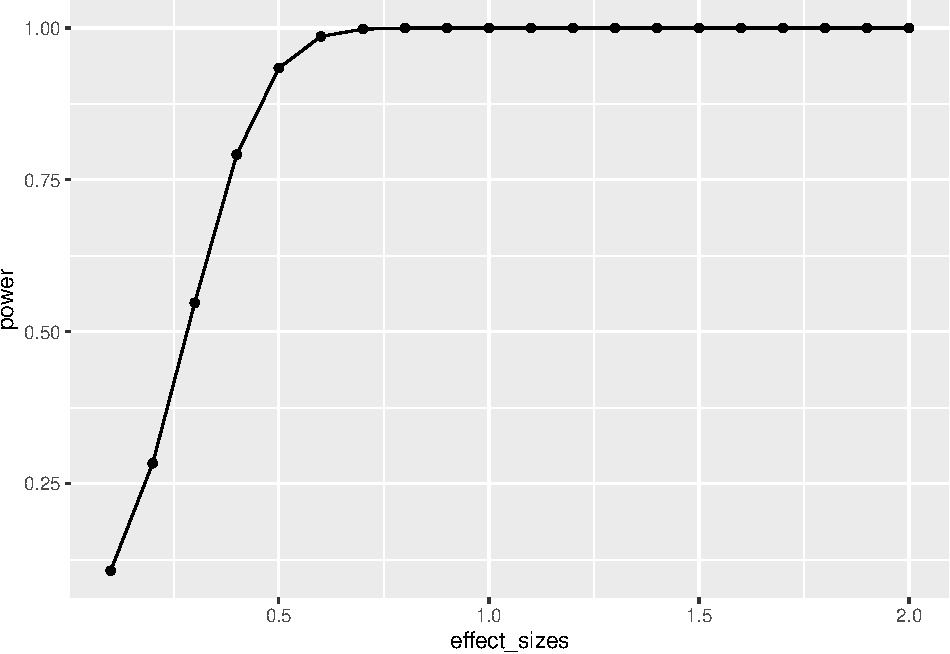
\includegraphics{SemesterProject_files/figure-latex/unnamed-chunk-4-1.pdf}
\caption{\label{fig:unnamed-chunk-4}A power curve analysis for a paired sample t-test with 50 participants.}
\end{figure}

\newpage

\hypertarget{references}{%
\section{References}\label{references}}

\begingroup
\setlength{\parindent}{-0.5in}
\setlength{\leftskip}{0.5in}

\hypertarget{refs}{}
\begin{CSLReferences}{1}{0}
\leavevmode\vadjust pre{\hypertarget{ref-bugg2012support}{}}%
Bugg, J. M., \& Crump, M. J. (2012). In support of a distinction between voluntary and stimulus-driven control: A review of the literature on proportion congruent effects. \emph{Frontiers in Psychology}, \emph{3}, 367.

\leavevmode\vadjust pre{\hypertarget{ref-macleod1991half}{}}%
MacLeod, C. M. (1991). Half a century of research on the stroop effect: An integrative review. \emph{Psychological Bulletin}, \emph{109}(2), 163.

\leavevmode\vadjust pre{\hypertarget{ref-rosenbaum2017stand}{}}%
Rosenbaum, D., Mama, Y., \& Algom, D. (2017). Stand by your stroop: Standing up enhances selective attention and cognitive control. \emph{Psychological Science}, \emph{28}(12), 1864--1867.

\end{CSLReferences}

\endgroup


\clearpage
\renewcommand{\listfigurename}{Figure captions}


\end{document}
